
\documentclass[12pt]{article}

\usepackage{graphicx} 
\usepackage{geometry} 
\usepackage{pdfpages}


\geometry{
  a4paper,
  left=25mm,
  right=25mm,
  top=25mm,
  bottom=25mm
}

% Title 
\title{
    \vspace{2in} % Adjust vertical spacing
    \Huge \textbf{World Population Data Analysis Report} \\
    \vspace{0.5in} % Adjust vertical spacing
    \Large \textit{Only EDA} \\
    \vspace{1in} % Adjust vertical spacing
}

\author{
    Author
    \vspace{0.1in} \\
    \textbf{Lahiru Sadakelum} \\
    \vspace{0.5in} \\
}

\date{\today}

\begin{document}

\maketitle

\thispagestyle{empty} 

\newpage

\vspace{0.2in} 
\begin{center}
\Large
\textbf{Abstract}
\vspace{0.1in} 
\end{center}
        \large
       This report presents a detailed analysis of world population data since 1970. The primary objective is to understand world population trends and their implications. The analysis covers key metrics such as population growth rate, distribution, and geographic variations. We use data from reputable resources. We found various patterns through statistical and visualization methods. This report aims to provide some valuable information for researchers and the general public to better understand the world population

\vspace{0.9in} 
\begin{center}
\Large
\textbf{Introduction}
\vspace{0.1in} 
\end{center}
    Understanding global population dynamics is crucial for policymakers, researchers, and organizations to formulate informed strategies and policies. The world population has experienced significant growth and transformation, influenced by factors such as fertility rates, mortality rates, migration patterns, and socio-economic development. Analyzing these trends helps in anticipating future challenges and opportunities related to healthcare, education, employment, and environmental sustainability.\vspace{0.08in} 

    In this report, we utilize data from the United Nations World Population Prospects 2022 and other reputable sources to examine historical trends, regional disparities, and demographic projections. The analysis focuses on key metrics such as population size, growth rates, age structure, and geographical distribution, aiming to provide a comprehensive overview of global demographic patterns and their implications for the future.

\newpage
\vspace{1in} 
\begin{center}
\Large
\textbf{Methodology}
\vspace{0.1in} \\
\Large \vspace{0.1in} Data cleaning and EDA processes are below.
\end{center}

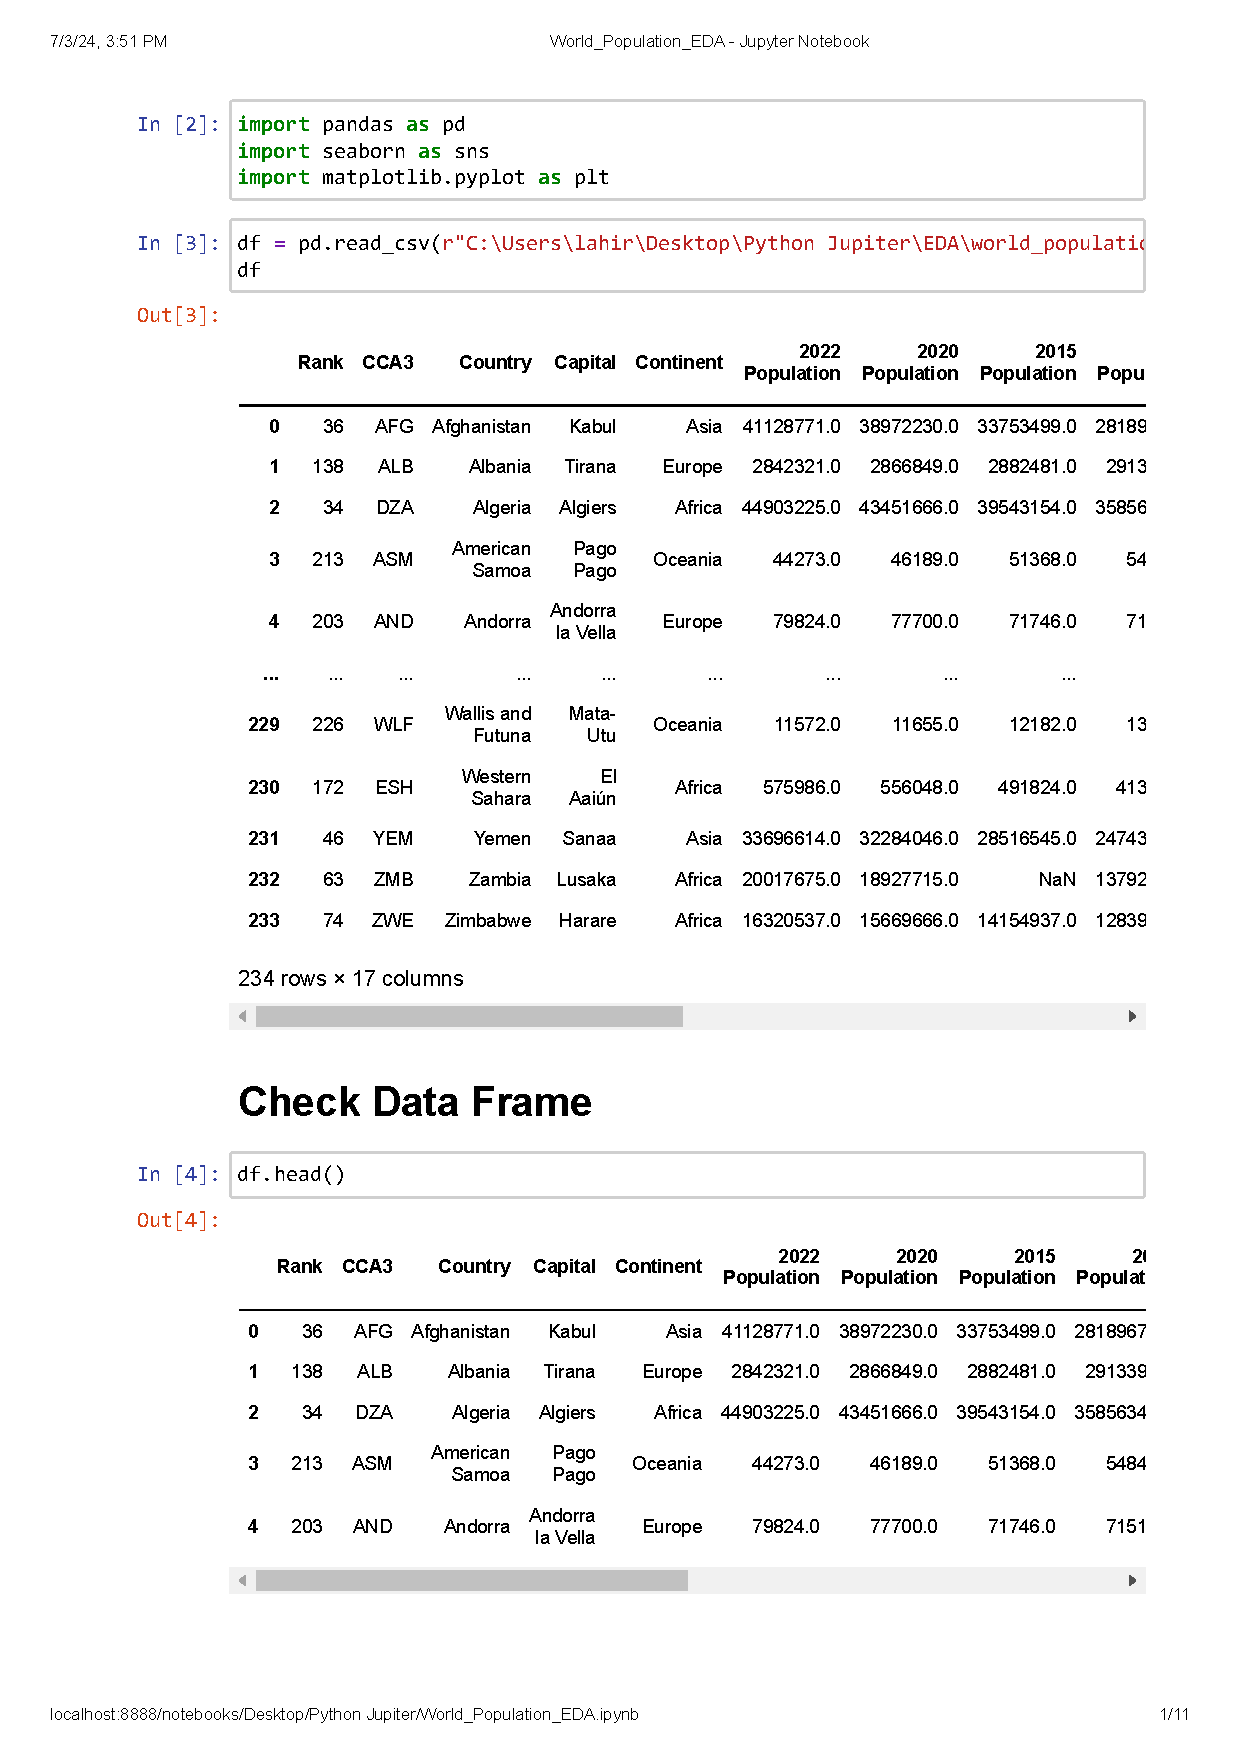
\includepdf[pages=-]{World_Population_EDA Project.pdf}

\newpage

\vspace{0.9in} 
\begin{center}
\Large
\textbf{Conclusion}
\vspace{0.1in} 
\end{center}
In conclusion,
    The global population has grown steadily, with significant regional disparities. Asia remains the most populous continent, while Africa exhibits the highest growth rates. These trends underscore the need for region-specific policies addressing population management and resource allocation.

\end{document}











